\documentclass[border=10pt]{standalone}
\usepackage[svgnames]{xcolor}
\usepackage{amsmath}
\usepackage{pgfplots}
\pgfplotsset{compat=newest}
\usepackage[sfdefault]{FiraSans}
\usepackage{FiraMono}
\renewcommand*\familydefault{\sfdefault}
\begin{document}
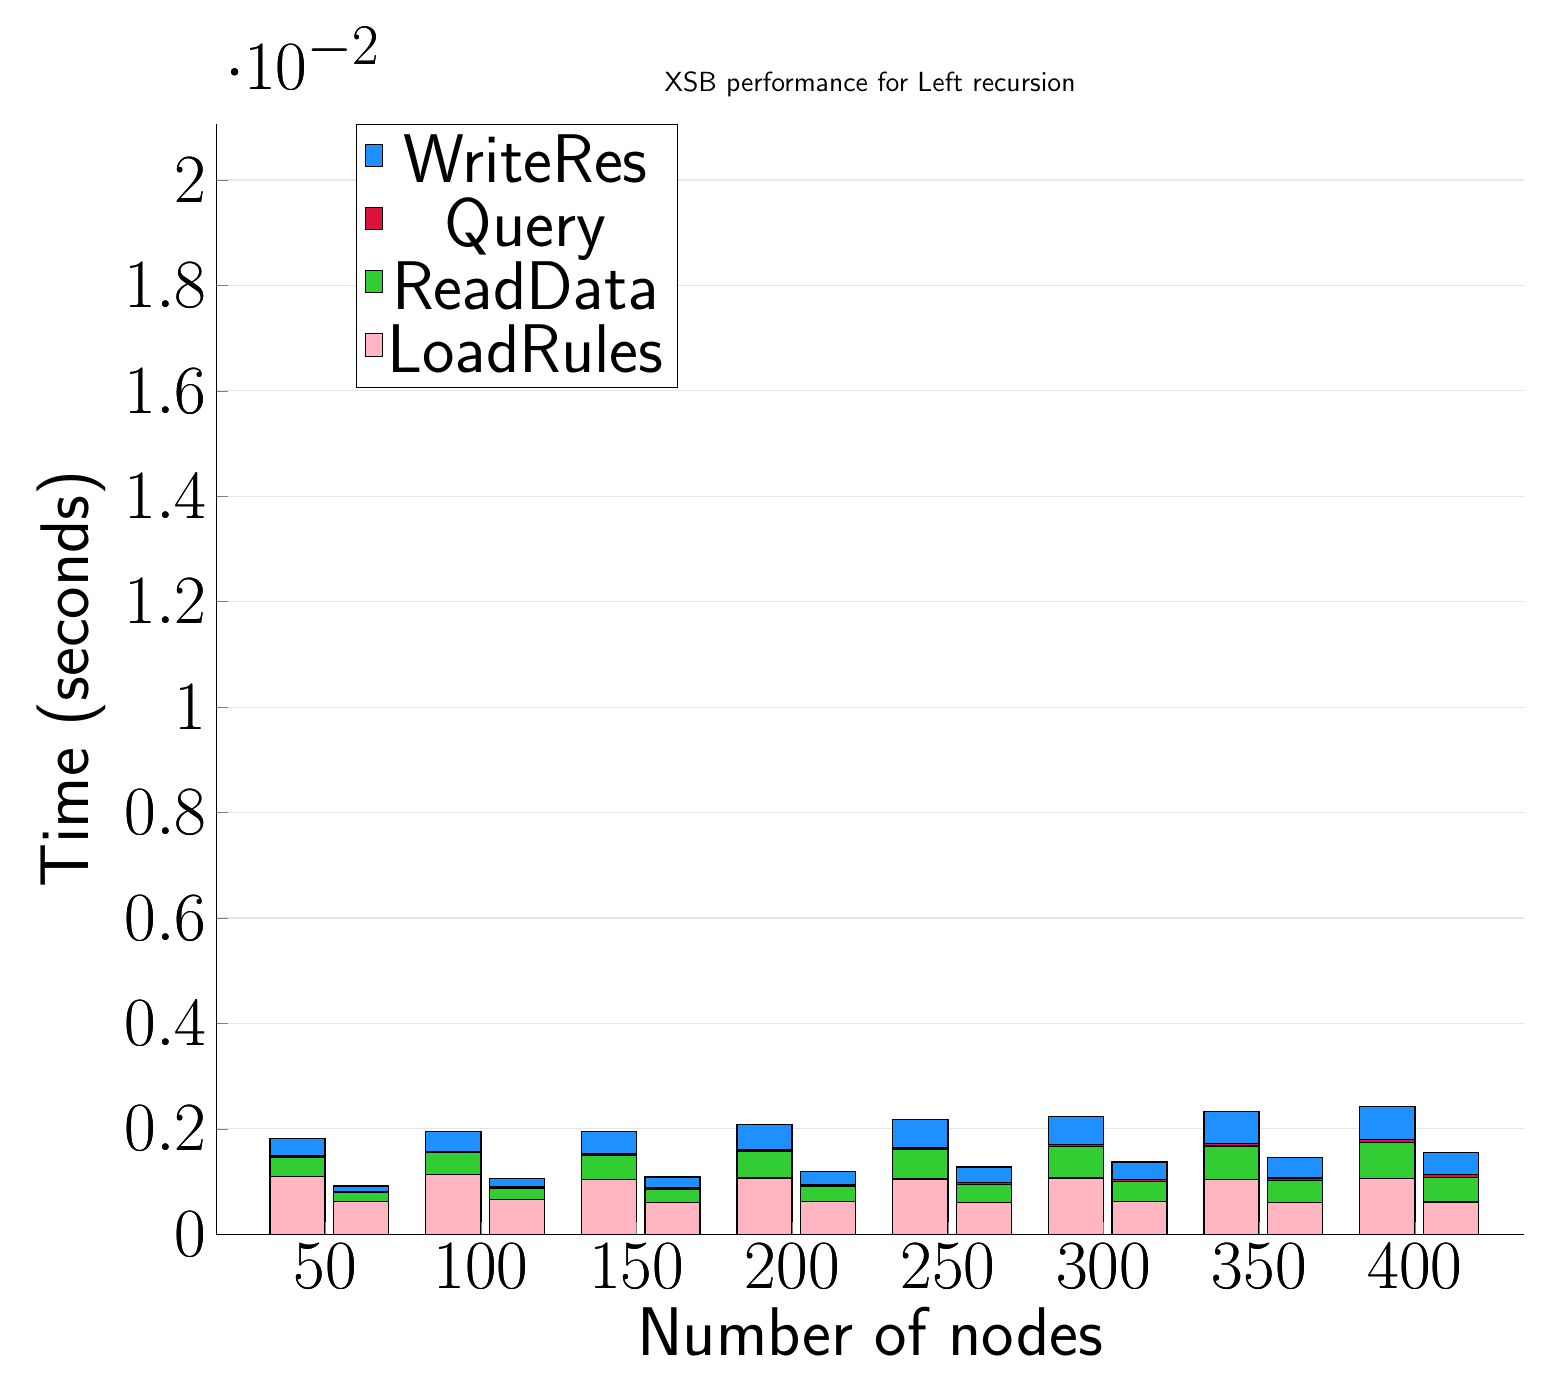
\begin{tikzpicture}
\begin{axis}[
   ybar stacked,
   title={XSB performance for Left recursion},
   bar shift=-10pt,
   width=1.5\textwidth,
   bar width=0.7cm,
   ymajorgrids, tick align=inside,
   major grid style={draw=gray!20},
   xtick=data,
   ymin=0, ymax=0.021072192192077635,
   axis x line*=bottom,
   axis y line*=left,
   enlarge x limits=0.1,
   legend style={
       at={(0.23, 1)},
       anchor=north,
       legend columns=1,
       font=\Huge,
   },
   ylabel={Time (seconds)},
   xlabel={Number of nodes},
   label style={font=\Huge},
   tick label style={font=\Huge},
]
\addlegendimage{fill=DodgerBlue, draw=black, line width=0.2pt}
\addlegendentry{WriteRes}
\addlegendimage{fill=Crimson, draw=black, line width=0.2pt}
\addlegendentry{Query}
\addlegendimage{fill=LimeGreen, draw=black, line width=0.2pt}
\addlegendentry{ReadData}
\addlegendimage{fill=LightPink, draw=black, line width=0.2pt}
\addlegendentry{LoadRules}
\addplot +[fill=LightPink, draw=black, line width=0.5pt] coordinates {
    (50, 0.001099967956542968)
    (100, 0.0011286973953247071)
    (150, 0.001040124893188476)
    (200, 0.0010651111602783178)
    (250, 0.0010507106781005862)
    (300, 0.001066541671752929)
    (350, 0.001041054725646972)
    (400, 0.001058626174926756)
};
\addplot +[fill=LimeGreen, draw=black, line width=0.5pt] coordinates {
    (50, 0.000364518165588379)
    (100, 0.000421261787414551)
    (150, 0.0004535675048828127)
    (200, 0.0004997014999389649)
    (250, 0.0005512237548828125)
    (300, 0.0005923032760620115)
    (350, 0.0006350994110107423)
    (400, 0.0006810665130615232)
};
\addplot +[fill=Crimson, draw=black, line width=0.5pt] coordinates {
    (50, 1.8000602722167962e-05)
    (100, 2.41518020629883e-05)
    (150, 2.7728080749511718e-05)
    (200, 3.409385681152343e-05)
    (250, 3.697872161865231e-05)
    (300, 4.5180320739746094e-05)
    (350, 4.9734115600585936e-05)
    (400, 5.8984756469726564e-05)
};
\addplot +[fill=DodgerBlue, draw=black, line width=0.5pt] coordinates {
    (50, 0.00033702850341796873)
    (100, 0.0003693342208862303)
    (150, 0.0004258394241333007)
    (200, 0.00048046112060546876)
    (250, 0.0005388259887695312)
    (300, 0.0005300283432006838)
    (350, 0.0005999088287353516)
    (400, 0.000619029998779297)
};
\end{axis}
\begin{axis}[
   ybar stacked,
   bar shift=13pt,
   width=1.5\textwidth,
   bar width=0.7cm,
   ymajorgrids, tick align=inside,
   major grid style={draw=none},
   xtick=data,
   ymin=0, ymax=0.021072192192077635,
   axis x line*=none,
   axis y line*=none,
   enlarge x limits=0.1,
   label style={font=\Huge},
   tick label style={font=\Huge},
]
\addplot +[fill=LightPink, draw=black, line width=0.5pt] coordinates {
    (50, 0.0006180999999999999)
    (100, 0.0006551999999999997)
    (150, 0.0006023999999999997)
    (200, 0.0006176000000000004)
    (250, 0.0006039)
    (300, 0.0006185000000000002)
    (350, 0.0006024)
    (400, 0.0006145999999999999)
};
\addplot +[fill=LimeGreen, draw=black, line width=0.5pt] coordinates {
    (50, 0.00017330000000000042)
    (100, 0.0002231000000000001)
    (150, 0.00025680000000000006)
    (200, 0.0002938999999999999)
    (250, 0.00033989999999999986)
    (300, 0.00037799999999999997)
    (350, 0.0004173000000000002)
    (400, 0.00046300000000000003)
};
\addplot +[fill=Crimson, draw=black, line width=0.5pt] coordinates {
    (50, 1.3700000000000179e-05)
    (100, 2.0100000000000146e-05)
    (150, 2.3800000000000036e-05)
    (200, 2.829999999999983e-05)
    (250, 3.2400000000000306e-05)
    (300, 3.950000000000029e-05)
    (350, 4.559999999999996e-05)
    (400, 5.3200000000000114e-05)
};
\addplot +[fill=DodgerBlue, draw=black, line width=0.5pt] coordinates {
    (50, 0.00011319999999999972)
    (100, 0.00016119999999999993)
    (150, 0.00020309999999999968)
    (200, 0.00025250000000000045)
    (250, 0.00029769999999999976)
    (300, 0.00033709999999999936)
    (350, 0.00038769999999999994)
    (400, 0.00042450000000000007)
};
\end{axis}
\end{tikzpicture}

\end{document}
